\section{ABORDAGENS PSICOLÓGICAS}
\label{sec:abordagensPsicologicas}

Por tratar-se de uma área focada ao estudo da psique humana, a psicologia possui inúmeras bases de estudo, onde cada escola baseia-se para aplicar os seus estudos e trabalhos de maneira distinta. Cada abordagem possui sua própria contribuição para o avanço e entendimento da mente humana, utilizando seus vários caminhos de atuação para descrever o ser humano de maneira diferenciada \cite{Anhanguera2022}.

Todo profissional psicólogo trabalha baseando-se em uma abordagem, guiando sua forma de atuação com o paciente e os pontos apresentados ao longo das sessões, ou seja, são linhas teóricas que o profissional utiliza para conduzir seu trabalho com a psicoterapia. Nesse contexto, um ponto imprescindível a ser ressaltado é a inexistência de abordagens certas ou erradas, a escolha, tanto pelo profissional quanto pelo paciente, irá depender da cosmovisão exclusiva de cada ser humano \cite{Barros2022}.

\subsection{Psicanálise}
\label{sec:psicanalise}
A psicanálise origina-se no século XX como um dos motores alomórficos à medicina convencional da época, trazendo principalmente inovação e expansão no atendimento do paciente. Sua origem está diretamente relacionada à vida de seu principal fundador, Sigmund Freud, que colaborado pelo médico vienense Joseph Breuer, buscou denominar a composição da mente humana e explicar a gênese dos fenômenos histéricos (neurose, psicose e histeria), perturbações aparentemente físicas que possuem origem psíquica \cite{Clinica2017}.

O início da psicanálise está na determinação do conceito de "inconsciente", principalmente através do atendimento clínico de Anna O., jovem com dotes intelectuais elevados de vinte e um anos, que sofria de um quadro de histeria clássico: alterações psíquicas, paralisia, perturbações dos movimentos oculares, repugnância a alimentos e tosse nervosa. Nesse contexto, as experiências traumáticas eram retomadas inconscientemente pelo paciente através do processo de hipnose, onde o analista realizava suas avaliações e colhia informações relatadas pelo paciente. O livro "Estudos sobre a histeria", publicado por Freud e Breuer em 1895 descreve este e outros quatro casos similares de histeria, constituindo os primeiros trabalhos de impacto sobre essa vertente de estudo psicólogica \cite{Clinica2017}.

De acordo com \citeonline{Carnier2021}, dentro dessa vertente, a teoria do aparelho psíquico, ou seja, a interpretação da mente e do comportamento humano e suas correlações pode ser melhor representado por um iceberg, conforme demonstra a Figura 1:

\begin{figure}[H]
    \centering
    \caption{Aparelho psíquico da psicanálise.}
    \label{fig:aparelhoPsiquicoPsicanalise}
    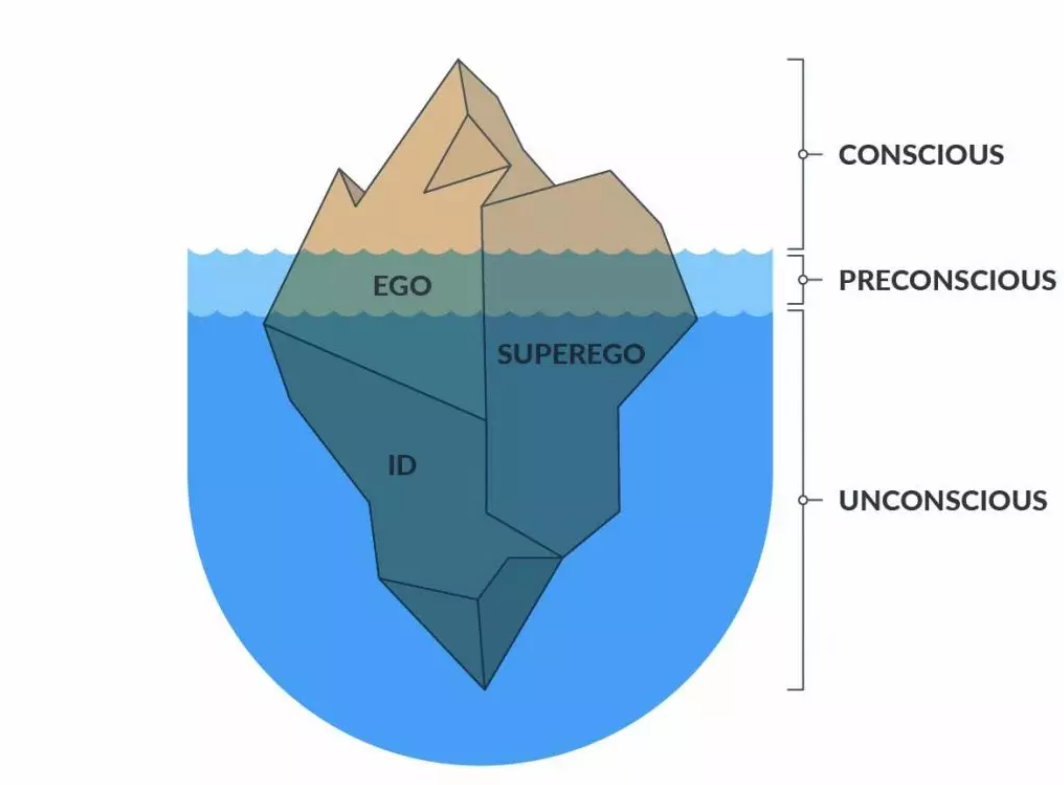
\includegraphics[width=.8\textwidth]{data/figures/psicanalise.png}
    \fonte{\citeonline{Carnier2021}}
\end{figure}

Ainda de acordo com \citeonline{Carnier2021}, a mente humana (tópicos à direita do iceberg) é dividida entre três partes:
\begin{itemize}
    \item \textbf{Consciente -} Corresponde a tudo aquilo que podemos perceber e acessar de forma intencional, ele é regido de acordo com as regras sociais, isto é, por meio dele é que se dá a nossa relação com o mundo;
    \item \textbf{Pré-consciente -} Se refere aos conteúdos que podem facilmente chegar ao consciente mas que não o permanecem, pode-se assemelhá-lo à uma peneira, filtrando as informações que transitam entre as outras duas camadas;
    \item \textbf{Inconsciente -} Representa qualquer conteúdo que não está na consciência, armazenando assim quase todas memórias consideradas perdidas, como nomes, sentimentos e medos.
\end{itemize}

Além disso, o mesmo autor ainda explicita as estruturas da personalidade humana (tópicos dentro do iceberg), constam três componentes distintos:
\begin{itemize}
    \item \textbf{Id -} Estrutura que fica na superfície, regindo nossa vida e comportamento na primeira infância, também é a estrutura que busca o prazer imediato, guiando-se pelos instintos e impulsos mais primitivos da nossa essência;
    \item \textbf{Ego -} Componente desenvolvido durante os 3 ou 4 anos de idade para lidar com conceitos de realidade e adaptação ao ambiente, é o aspecto racional da personalidade, controladora do "id";
    \item \textbf{Superego - } Entidade psíquica que surge a partir da socialização e das pressões impostas pelo contexto social e normas em que estamos inseridos, representando assim o aspecto moral da personalidade. 
\end{itemize}

Estes conceitos entrelaçam-se para dar a explicação de inúmeros conceitos da psicanálise, como as possíveis manifestações do ego (ego inflado, ego frágil, ego forte, dentre outros), como o princípio do prazer e como o ato falho.

\subsection{Humanismo}
\label{sec:Humanismo}
A terapia humanista tem origem na década de 1950 como contraposto à psicanálise e ao behaviorismo, defendendo que o indivíduo não é regido por um inconsciente e nem por fatores externos. O passo inicial do humanismo está nos pressupostos do psicólogo americano Abraham Malow, criador da "pirâmide de necessidades" \cite{Pimenta2019}, o diagrama sugere que há uma tendência humana natural de satisfazer necessidades mais prioritárias antes de atender outras mais específicas, e que desbalanceamentos em qualquer nível resulta em disformidade na pirâmide inteira \cite{Mcleod2023}.

\begin{figure}[H]
    \centering
    \caption{Pirâmide de Necessidades de Maslow.}
    \label{fig:piramideDeNecessidades}
    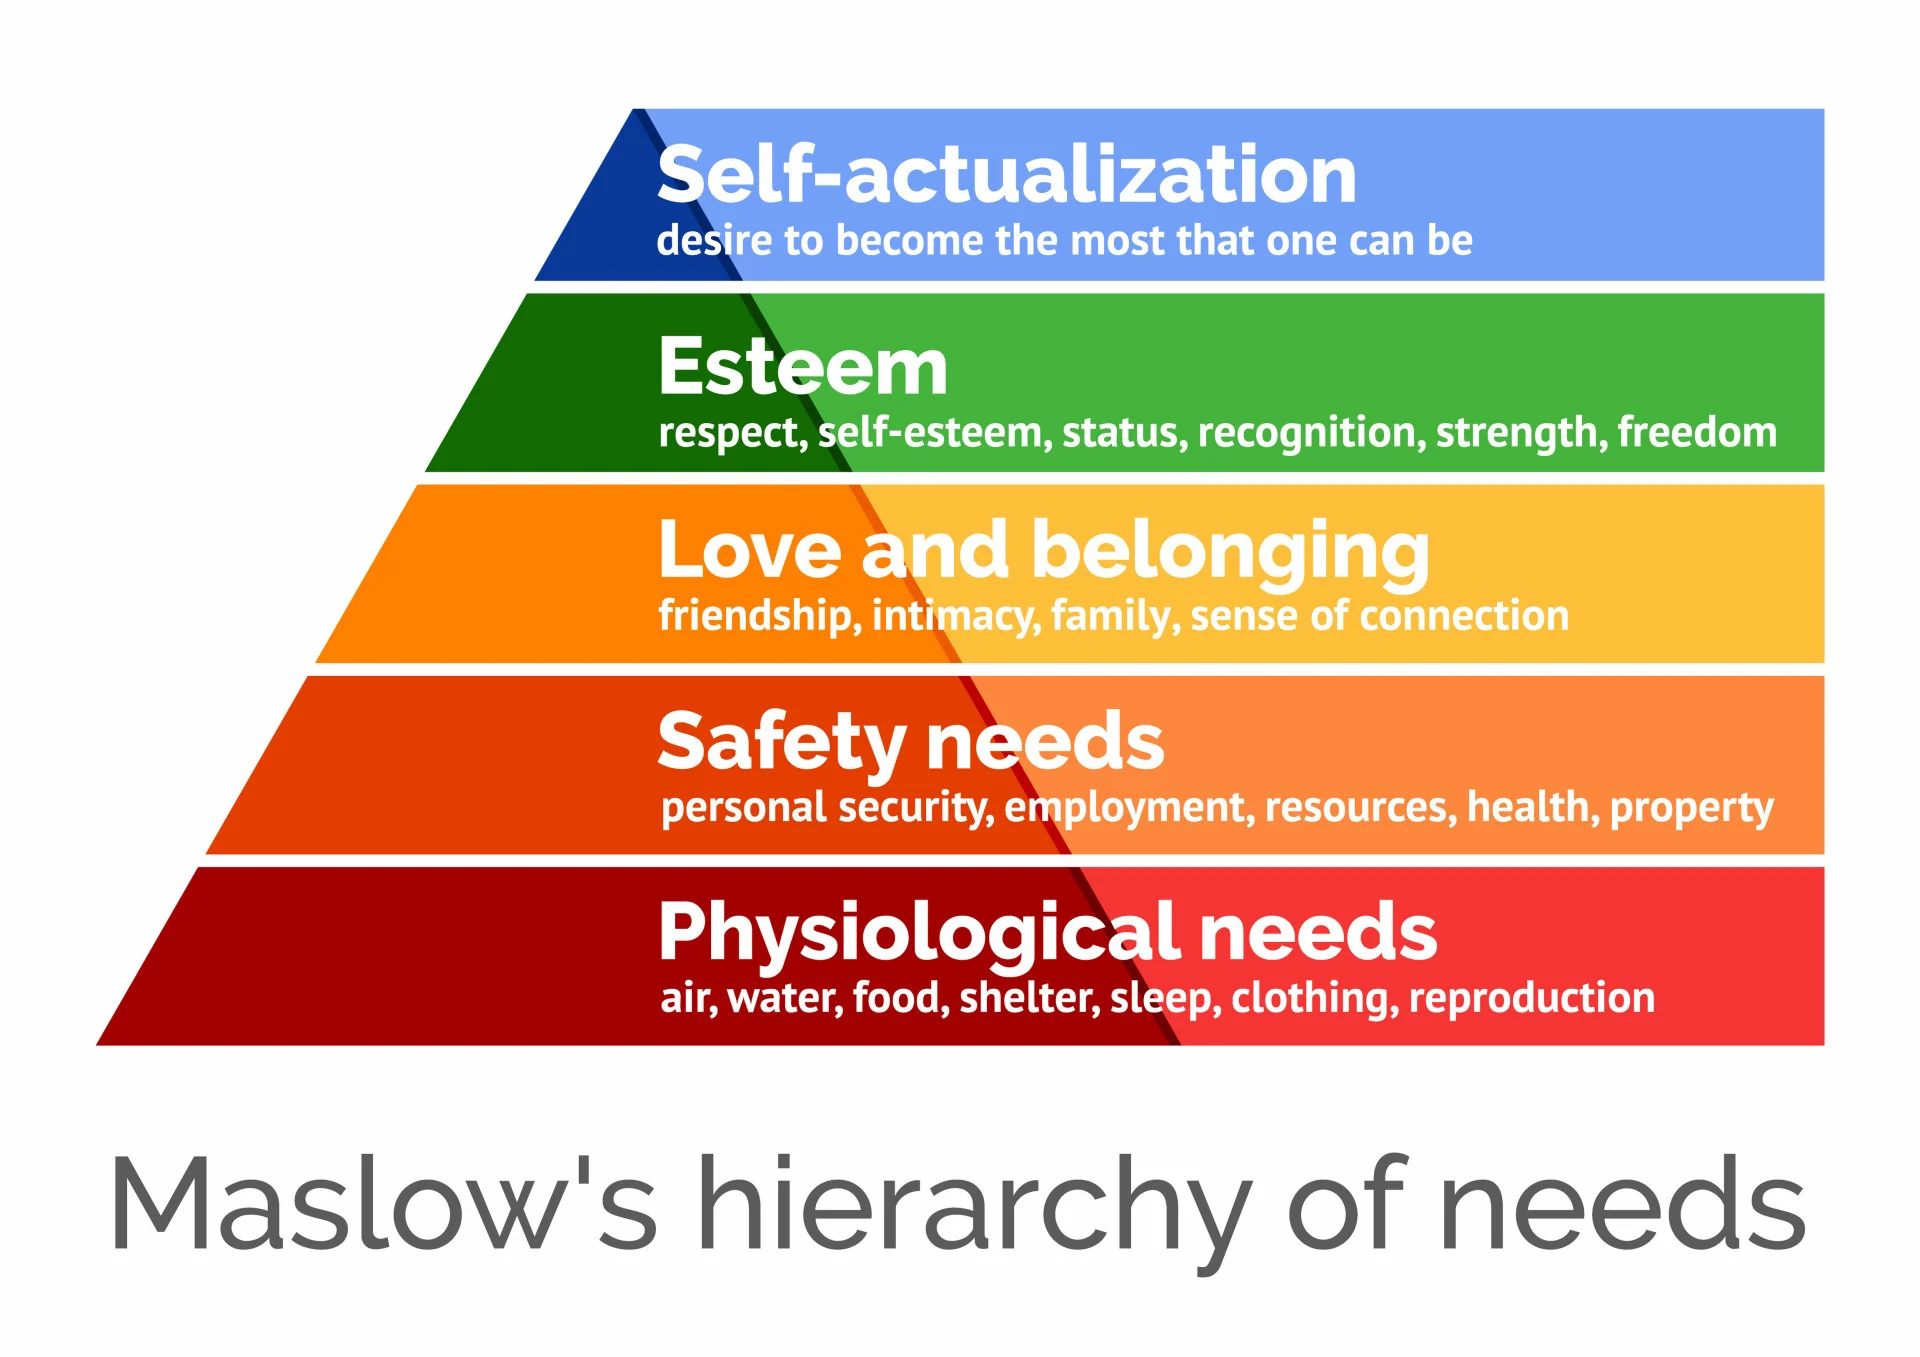
\includegraphics[width=.8\textwidth]{data/figures/piramide-de-necessidades.png}
    \fonte{\citeonline{Mcleod2023}}
\end{figure} 

Inspirado por isso, em 1951, Carl Rogers publicou o livro "Terapia Centrada ao Cliente", contendo sua primeira teoria formal da terapia e da teoria da formalidade, além de algumas pesquisas que ressaltavam seus argumentos. Segundo o psicólogo, para uma pessoa "crescer" e se autorrealizar, é necessário um ambiente que lhe proporcione verdade (abertura e revelação), aceitação (ser aceito incondicionalmente como é) e empatia (ser compreendido). Segundo o autor, sem possuir isso, personalidades e relacionamentos não se desenvolvem de forma saudável \cite{Pimenta2019}.

O humanismo procura aproximar a relação entre cliente e terapeuta, tornando o processo da psicoterapia o mais humanizado possível, partindo sempre do princípio da aceitação incondicional. Nessa vertente, há uma inversão de valores, onde o cliente é o foco da terapia, e não mais o profissional. Para reforçar ainda mais essa aproximação, a utilização da palavra "cliente" também é reforçada, uma vez que, segundo Rogers, a palavra "paciente" possui uma conotação desnecessariamente debilitante, já que remete a uma pessoa doente, que necessita de cuidados e que não pode responder a si \cite{Barros2022}.

Para o autor, o indivíduo possui o desejo básico e capacidade de se autorrealizar, isto é, atingir o nível mais elevado possível de seu próprio potencial. Porém, a capacidade de executar essa tarefa pode estar adormecida e precisa ser despertada, alcançando isso através da abordagem terapêutica humanista, auxíliada por um psicólogo. Nesse contexto, o profissional deve guiar o cliente sem julgá-lo a uma estratégia sem antes fazer uma confrontação. Ainda de acordo com Rogers, o objetivo do humanismo era escutar o cliente, facilitar seu autoconhecimento e ajudá-lo a encontrar sua definição de personalidade \cite{Pimenta2019}.

Nessa vertente utiliza-se muito do diálogo, incentivando veemente o cliente a se expressar. Sua aplicação encontra-se sim no tratamento de indivíduos com transtornos mentais, mas também inclui ajudar as pessoas a explorarem seus pontos fortes e descobrir suas habilidades e objetivos. A terapia humanista explora os pontos fortes de cada indivíduo, e trata cada um com familiaridade, sem posições de autoridade ou de julgamento. Acolhendo o ser, e procurando mostrá-lo suas próprias vontades e como buscar satisfação pessoal com êxito \cite{Brandao2023}.

\subsection{Sistêmica}
\label{sec:sistemica}
A abordagem sistêmica baseia-se na Teoria Geral dos Sistemas, que surgiu na década de 1950. Essa ramificação busca entender as pessoas a partir das interações e relações que estabelecem com o ambiente e com outros indivíduos ao seu redor, considerando e analisando assim o indivíduo como parte de um sistema (família, grupo social ou organização). A premissa básica está em considerar que as relações entre os indivíduos afetam diretamente a saúde mental de cada um, e que problemáticas podem ter origem no sistema, e não diretamente no indivíduo singular \cite{Verissimo2020}.

Na aplicação desta abordagem, o profissional utiliza de inúmeras outras abordagens para analisar os sistemas sociais que se conectam complexamente. Torna-se um processo cíclico, onde analisa-se ao mesmo tempo o indivíduo e o sistema, não podendo compreender todo o sistema sem compreender as partes e vice-versa. Ao fim, evidentemente, a sistêmica atua de maneira mais proativa na prevenção e tratamento de perturbações mentais \cite{Psychotherapy2009}. 

Dada a forma como nos relacionamos sistematicamente, muitos de nossos empecilhos acabam por trazer os males psíquicos que enfrentamos. Nisso, trabalha-se principalmente a parte psicossocial do paciente, aplicando recursos que ajudem no desenvolvimento do indivíduo de forma individual e dentro de um contexto social. Partindo de tudo isso, o desenvolvimento trabalhado ajuda a fazer a integração dos sistemas, unificando as partes necessárias ao crescimento. A mudança vem do individual, se espalha ao restante do sistema e retorna ao seu início, reciclando-se continuamente \cite{Verissimo2020}.

Consequentemente, por tratar especialmente o sistema como um todo, a abordagem sistêmica atua principalmente em terapia conjugal e familiar, buscando explorar e entender os padrões de comunicação e relacionamento inerentes a esse grupo. Além de também atuar em quaisquer organizações comunitaŕias, englobando assim toxicodependência, reclusão e alcoolismo \cite{Psychotherapy2009}.

\subsection{Cognitivo-Comportamental}
\label{sec:cognitivoComportamental}
A terapia cognitivo comportamental (TCC) teve início na década de 1960 com os estudos do psiquiatra Aaron Beck, sobre o qual acreditava que os fundamentos de seu trabalho necessitavam da validação científica para serem apresentados e aceitos pela comunidade médica. O nome dessa abordagem deriva dos processos e ferramentas que foram incorporadas nas estruturas das sessões com os pacientes \cite{Nogueira2018}.

Segundo Beck, a psicanálise, formato comum utilizado no tratamento de pacientes com depressão, era um processo muito duradouro que não trazia resultados satisfatórios. Partindo disso, o psiquiatra modificou a estrutura e modelo da psicoterapia, focando-a para o presente e para solução de problemas \cite{Barros2022}.

A base teórica da TCC aponta que nossas emoções e comportamentos são diretamente influenciados por nossos pensamentos. Quaisquer eventos que presenciamos promovem ativações de pensamento, resultando em uma resposta emocional, e por consequência afeta o comportamento. Nesse contexto, as distorções cognitivas ou distorções de pensamentos levam o indivíduo a chegar em conclusões equivocadas sobre si mesmo e sobre o mundo ao seu redor \cite{Education2023}. Em outras palavras, segundo a vertente, com o paciente tornando o pensamento mais realista e saudável existe uma melhoria significativa em seu estado emocional, e por consequência, seu comportamento também é afetado. Por fim, criando assim um ciclo. 

\begin{figure}[H]
    \centering
    \caption{Ciclo da TCC.}
    \label{fig:cicloTCC}
    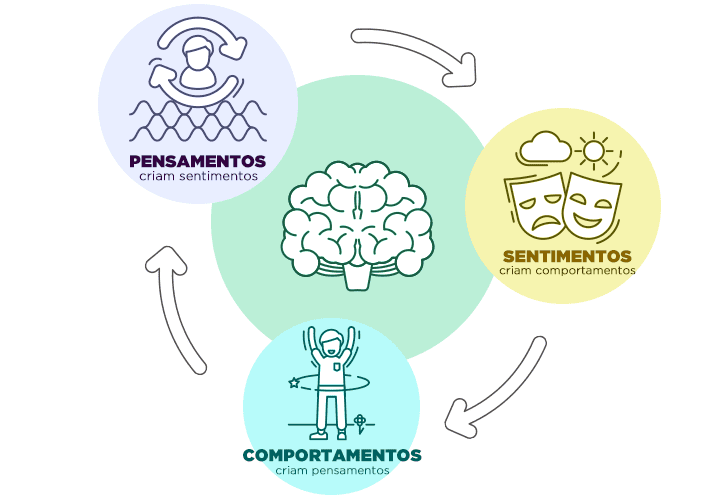
\includegraphics[width=.8\textwidth]{data/figures/tcc-esquema.png}
    \fonte{\citeonline{Education2023}}
\end{figure}

A psicoterapia em TCC é um trabalho colaborativo entre paciente e profissional, onde o paciente representa um papel mais ativo durante as sessões, fazendo os exercícios propostos pelo psicólogo e dando feedbacks constantes ao terapeuta. Ao mesmo tempo, essa vertente emprega estratégias cognitivas e comportamentais para o paciente focar em aspectos mais saudáveis da vida e das suas metas pessoais, priorizando assim, o seu bem estar \cite{Education2023}.